\documentclass[a4paper]{article}
\usepackage{inputenc}
\usepackage[british,UKenglish]{babel}
\usepackage{amsmath}
%\usepackage{titlesec}
\usepackage{color}
\usepackage{graphicx}
\usepackage{fancyref}
\usepackage{hyperref}
\usepackage{float}
\usepackage{scrextend}
\usepackage{setspace}
\usepackage{xargs}
\usepackage{multicol}
\usepackage{nameref}

\usepackage{sectsty}
\usepackage{multicol}
\usepackage{multirow}
\usepackage[procnames]{listings}
\usepackage{appendix}

\newcommand\tab[1][1cm]{\hspace*{#1}}
\hypersetup{colorlinks=true, linkcolor=black}
\interfootnotelinepenalty=10000

\newcommand{\cleancode}[1]{\begin{addmargin}[3em]{3em}\texttt{\textcolor{cleanOrange}{#1}}\end{addmargin}}
\newcommand{\cleanstyle}[1]{\text{\textcolor{cleanOrange}{\texttt{#1}}}}


\usepackage[colorinlistoftodos,prependcaption,textsize=footnotesize]{todonotes}
\newcommandx{\commred}[2][1=]{\textcolor{Red}
{\todo[linecolor=red,backgroundcolor=red!25,bordercolor=red,#1]{#2}}}
\newcommandx{\commblue}[2][1=]{\textcolor{Blue}
{\todo[linecolor=blue,backgroundcolor=blue!25,bordercolor=blue,#1]{#2}}}
\newcommandx{\commgreen}[2][1=]{\textcolor{OliveGreen}{\todo[linecolor=OliveGreen,backgroundcolor=OliveGreen!25,bordercolor=OliveGreen,#1]{#2}}}
\newcommandx{\commpurp}[2][1=]{\textcolor{Plum}{\todo[linecolor=Plum,backgroundcolor=Plum!25,bordercolor=Plum,#1]{#2}}}

\def\code#1{{\tt #1}}

\def\note#1{\noindent{\bf [Note: #1]}}

\makeatletter
%% The "\@seccntformat" command is an auxiliary command
%% (see pp. 26f. of 'The LaTeX Companion,' 2nd. ed.)
\def\@seccntformat#1{\@ifundefined{#1@cntformat}%
   {\csname the#1\endcsname\quad}  % default
   {\csname #1@cntformat\endcsname}% enable individual control
}
\let\oldappendix\appendix %% save current definition of \appendix
\renewcommand\appendix{%
    \oldappendix
    \newcommand{\section@cntformat}{\appendixname~\thesection\quad}
}
\makeatother


% "define" Scala
\usepackage[T1]{fontenc}  
\usepackage[scaled=0.82]{beramono}  
\usepackage{microtype} 

\sbox0{\small\ttfamily A}
\edef\mybasewidth{\the\wd0 }

\lstdefinelanguage{scala}{
  morekeywords={abstract,case,catch,class,def,%
    do,else,extends,false,final,finally,%
    for,if,implicit,import,match,mixin,%
    new,null,object,override,package,%
    private,protected,requires,return,sealed,%
    super,this,throw,trait,true,try,%
    type,val,var,while,with,yield},
  sensitive=true,
  morecomment=[l]{//},
  morecomment=[n]{/*}{*/},
  morestring=[b]",
  morestring=[b]',
  morestring=[b]"""
}

\usepackage{color}
\definecolor{dkgreen}{rgb}{0,0.6,0}
\definecolor{gray}{rgb}{0.5,0.5,0.5}
\definecolor{mauve}{rgb}{0.58,0,0.82}

% Default settings for code listings
\lstset{frame=tb,
  language=scala,
  aboveskip=3mm,
  belowskip=3mm,
  showstringspaces=false,
  columns=fixed, % basewidth=\mybasewidth,
  basicstyle={\small\ttfamily},
  numbers=none,
  numberstyle=\footnotesize\color{gray},
  % identifierstyle=\color{red},
  keywordstyle=\color{blue},
  commentstyle=\color{dkgreen},
  stringstyle=\color{mauve},
  frame=single,
  breaklines=true,
  breakatwhitespace=true,
  procnamekeys={def, val, var, class, trait, object, extends},
  procnamestyle=\ttfamily\color{red},
  tabsize=2
}

\lstnewenvironment{scala}[1][]
{\lstset{language=scala,#1}}
{}
\lstnewenvironment{cpp}[1][]
{\lstset{language=C++,#1}}
{}
\lstnewenvironment{bash}[1][]
{\lstset{language=bash,#1}}
{}
\lstnewenvironment{verilog}[1][]
{\lstset{language=verilog,#1}}
{}



\graphicspath{ {images/} }
\usepackage{ctex}
\usepackage{graphicx}
\usepackage{color,framed}%文本框
\usepackage{listings}
\usepackage{caption}

\usepackage{hyperref}
\hypersetup{hidelinks,
	colorlinks=true,
	allcolors=black,
	pdfstartview=Fit,
	breaklinks=true}


\lstdefinestyle{mystyle}{
  keywordstyle=\color{orange},  % 设置关键词颜色为橙色
 morekeywords={set, nmap, msfconsole,exploit},           % 仅将 set 设置为橙色
}

\usepackage{amssymb}
\usepackage{enumerate}
\usepackage{xcolor}
\usepackage{bm} 
\usepackage{lastpage}%获得总页数
\usepackage{fancyhdr}
\usepackage{tabularx}  
\usepackage{geometry}
\usepackage{minted}
\usepackage{graphics}
\usepackage{subfigure}
\usepackage{float}
\usepackage{pdfpages}
\usepackage{pgfplots}
\pgfplotsset{width=10cm,compat=1.9}
\usepackage{multirow}
\usepackage{footnote}
\usepackage{booktabs}
\usepackage{listings}

%-----------------------伪代码------------------
\usepackage{algorithm}  
\usepackage{algorithmicx}  
\usepackage{algpseudocode}  
\floatname{algorithm}{Algorithm}  
\renewcommand{\algorithmicrequire}{\textbf{Input:}}  
\renewcommand{\algorithmicensure}{\textbf{Output:}} 
\usepackage{lipsum}  
\makeatletter
\newenvironment{breakablealgorithm}
  {% \begin{breakablealgorithm}
  \begin{center}
     \refstepcounter{algorithm}% New algorithm
     \hrule height.8pt depth0pt \kern2pt% \@fs@pre for \@fs@ruled
     \renewcommand{\caption}[2][\relax]{% Make a new \caption
      {\raggedright\textbf{\ALG@name~\thealgorithm} ##2\par}%
      \ifx\relax##1\relax % #1 is \relax
         \addcontentsline{loa}{algorithm}{\protect\numberline{\thealgorithm}##2}%
      \else % #1 is not \relax
         \addcontentsline{loa}{algorithm}{\protect\numberline{\thealgorithm}##1}%
      \fi
      \kern2pt\hrule\kern2pt
     }
  }{% \end{breakablealgorithm}
     \kern2pt\hrule\relax% \@fs@post for \@fs@ruled
  \end{center}
  }
\makeatother
%------------------------代码-------------------
\RequirePackage{listings}
\RequirePackage{xcolor}
\definecolor{dkgreen}{rgb}{0,0.6,0}
\definecolor{gray}{rgb}{0.5,0.5,0.5}
\definecolor{mauve}{rgb}{0.58,0,0.82}
\lstset{
	numbers=left,  
	frame=tb,
	aboveskip=3mm,
	belowskip=3mm,
	showstringspaces=false,
	columns=flexible,
	framerule=1pt,
	rulecolor=\color{gray!35},
	backgroundcolor=\color{gray!5},
	basicstyle={\ttfamily},
	numberstyle=\tiny\color{gray},
	keywordstyle=\color{blue},
	commentstyle=\color{dkgreen},
	stringstyle=\color{mauve},
	breaklines=true,
	breakatwhitespace=true,
	tabsize=3,
}


%-------------------------页面边距--------------
\geometry{a4paper,left=2.5cm,right=2.5cm,top=2.6cm,bottom=2.7cm}
%-------------------------页眉页脚--------------
\usepackage{fancyhdr}
\pagestyle{fancy}
\lhead{\kaishu }
\chead{}
\rhead{{\CJKfontspec{simkai.ttf} }}
\lfoot{}
\cfoot{\thepage}
\rfoot{}
\renewcommand{\headrulewidth}{0pt}  
\renewcommand{\footrulewidth}{0pt}
\newcommand{\HRule}{\rule{\linewidth}{0.5mm}}
\newcommand{\HRulegrossa}{\rule{\linewidth}{1.2mm}}
\setlength{\textfloatsep}{10mm}
%--------------------文档内容--------------------
\renewcommand{\contentsname}{目\ 录}
\renewcommand{\appendixname}{附录}
\renewcommand{\appendixpagename}{附录}
\renewcommand{\refname}{参考文献} 
\renewcommand{\figurename}{图}
\renewcommand{\tablename}{表}
\renewcommand{\today}{\number\year 年 \number\month 月 \number\day 日}

\renewcommand {\thefigure}{\thesection{}.\arabic{figure}}%图片按章标号
\renewcommand{\figurename}{图}
\renewcommand{\contentsname}{目录}  
\cfoot{\thepage\ of \pageref{LastPage}}%当前页 of 总页数

\renewcommand{\abstractname}{\textbf{\Large 摘要}} % 调整摘要标题的字体大小
\renewcommand {\thefigure}{\thesection{}.\arabic{figure}}%图片按章标号

\begin{document}

\renewcommand{\figurename}{图}
\renewcommand{\contentsname}{目录}  
\cfoot{\thepage\ of \pageref{LastPage}}
\renewcommand{\abstractname}{\textbf{\Large 摘要}} 

\begin{center}
    \huge{\textbf{体系结构第二次实验报告}}
\end{center}

\begin{center}
    \textbf{姓名}:\underline{梁朝阳 2311561} \quad
    \textbf{专业}:\underline{密码科学与技术}
\end{center}

\tableofcontents

\vspace*{1cm}

\noindent{\Large\textbf{摘要}}

\vspace{1em}

\textbf{设计思路与架构:} 
旁路设计图见图2.1,设计思路在后面详细讲述,这里只是简单介绍架构:首先创建独立的bypass\_unit.v模块。主要的注意点在于优先级选取,和转移未完成的stall的检测。还有就是也对比了下我在国庆前的不完全正确实现(EXE阶段前递),说明了为什么我选择了ID阶段前递。

\textbf{代码实现:}没有完全按照CPU设计实战中的建议,而是采用了我自己的实现方式,主要是为了简化逻辑,避免冒险修改级联控制中ready\_go信号的复杂性(与出错的可能性),最后结果也是正确的。

\textbf{仿真对比效果:}从三个方面对比了仿真效果:整体直观上总周期变短;branch与乘法延迟情况,最后从细节举例确实减少了周期的指令。

\newpage

\section{实验要求}

请在第一次实验的五级流水线CPU的基础上,根据《CPU设计实战》这本书上第四章后面的内容,验证现有CPU的指令相关和流水线冲突问题,以添加旁路的方式和前递技术,让CPU规避这样的问题。注意:

\begin{enumerate}
    \item 实验报告中简要画一下旁路设计的示意图,有对应的介绍 。  
    \item 进行详细分析,原始情况下指令是如何执行的,增加了旁路和前递之后是如何执行的。
\end{enumerate}

\section{旁路设计图}

\begin{figure}[H]
    % \centering
    \hspace*{-0.9cm} % 根据需要调整此处的负值(如-4cm)实现左移,数值越大左移越多
    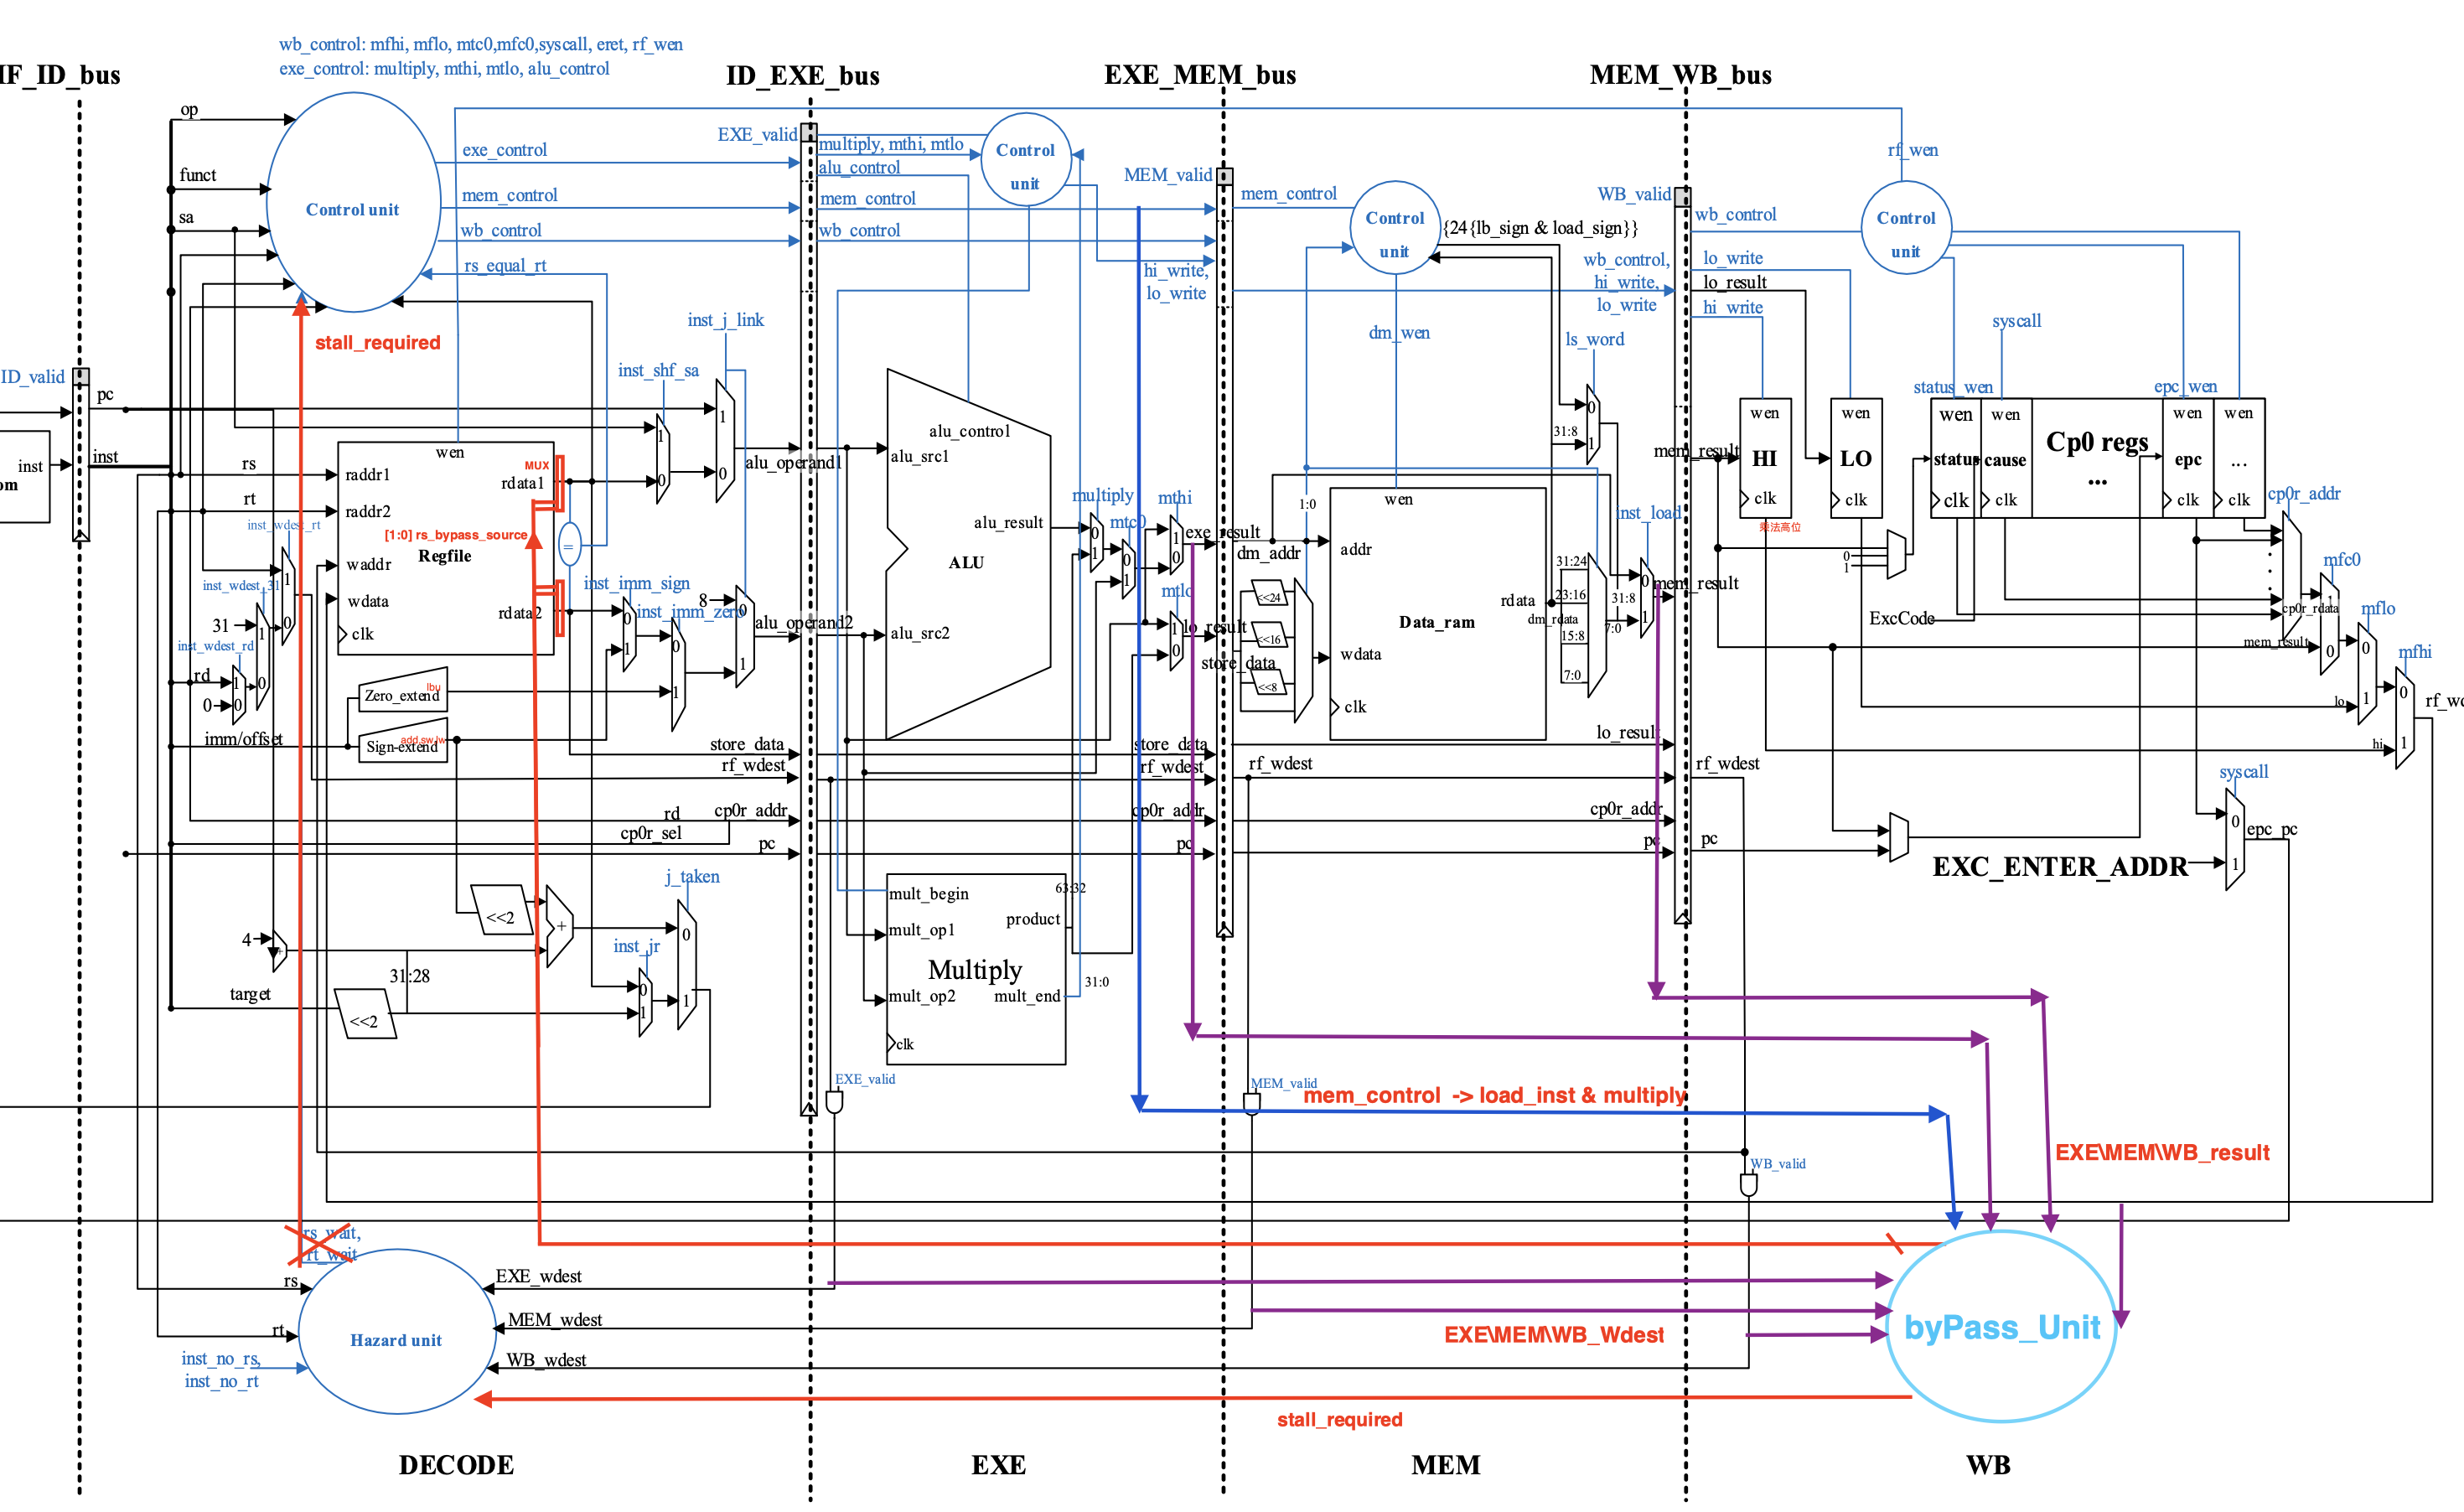
\includegraphics[width=1.1\linewidth]{img/旁路修改图片/旁路设计图.png}
    \caption{EXE/MEM/WB -> ID 旁路设计图}
\end{figure}

设计思路(为什么这么设计以及详细考量)在后面详细讲述,这里只是简单介绍架构:首先创建独立的bypass\_unit.v模块,ID选择操作数结果优先级:EXE > MEM > WB > 寄存器堆。且由于在ID阶段实现了branch,因此具有「转移计算未完成(load-branch)」这类特殊情况(需要stall)。因此我的旁路内对类似这种情况\footnote{实际上CPU设计书中说的不是特别全,还有乘法运算也同样需要检测。实际实现下来,我的做法是对所有branch前有运算相关性的都进行stall,下文会详细叙述原因。}进行了检测。

bypass\_unit考虑级联控制中的valid值接受EXE/MEM/WB阶段的写回地址Wdest与写回值(result)。同时接受mem\_control信号中的判断类型信号。最终输出rs\_bypass\_source 与 stall\_required,替代wait信号。

\newpage


\section{实验过程}

\subsection{设计思路(我的考虑与尝试)}

\subsubsection{前递阶段选取与转移计算未完成情况}

最开始选择了前递到EXE阶段,结果导致发现ID阶段的Branch指令难以处理(导致错误,因Branch也需要前递信息),要加更多非常复杂的控制信号,实现出来的稳定性与开销也不太好。尝试这个方向发现行不通之后,我回退版本,重新实现了全部前递到ID阶段的旁路:

\begin{figure}[H]
    \centering
    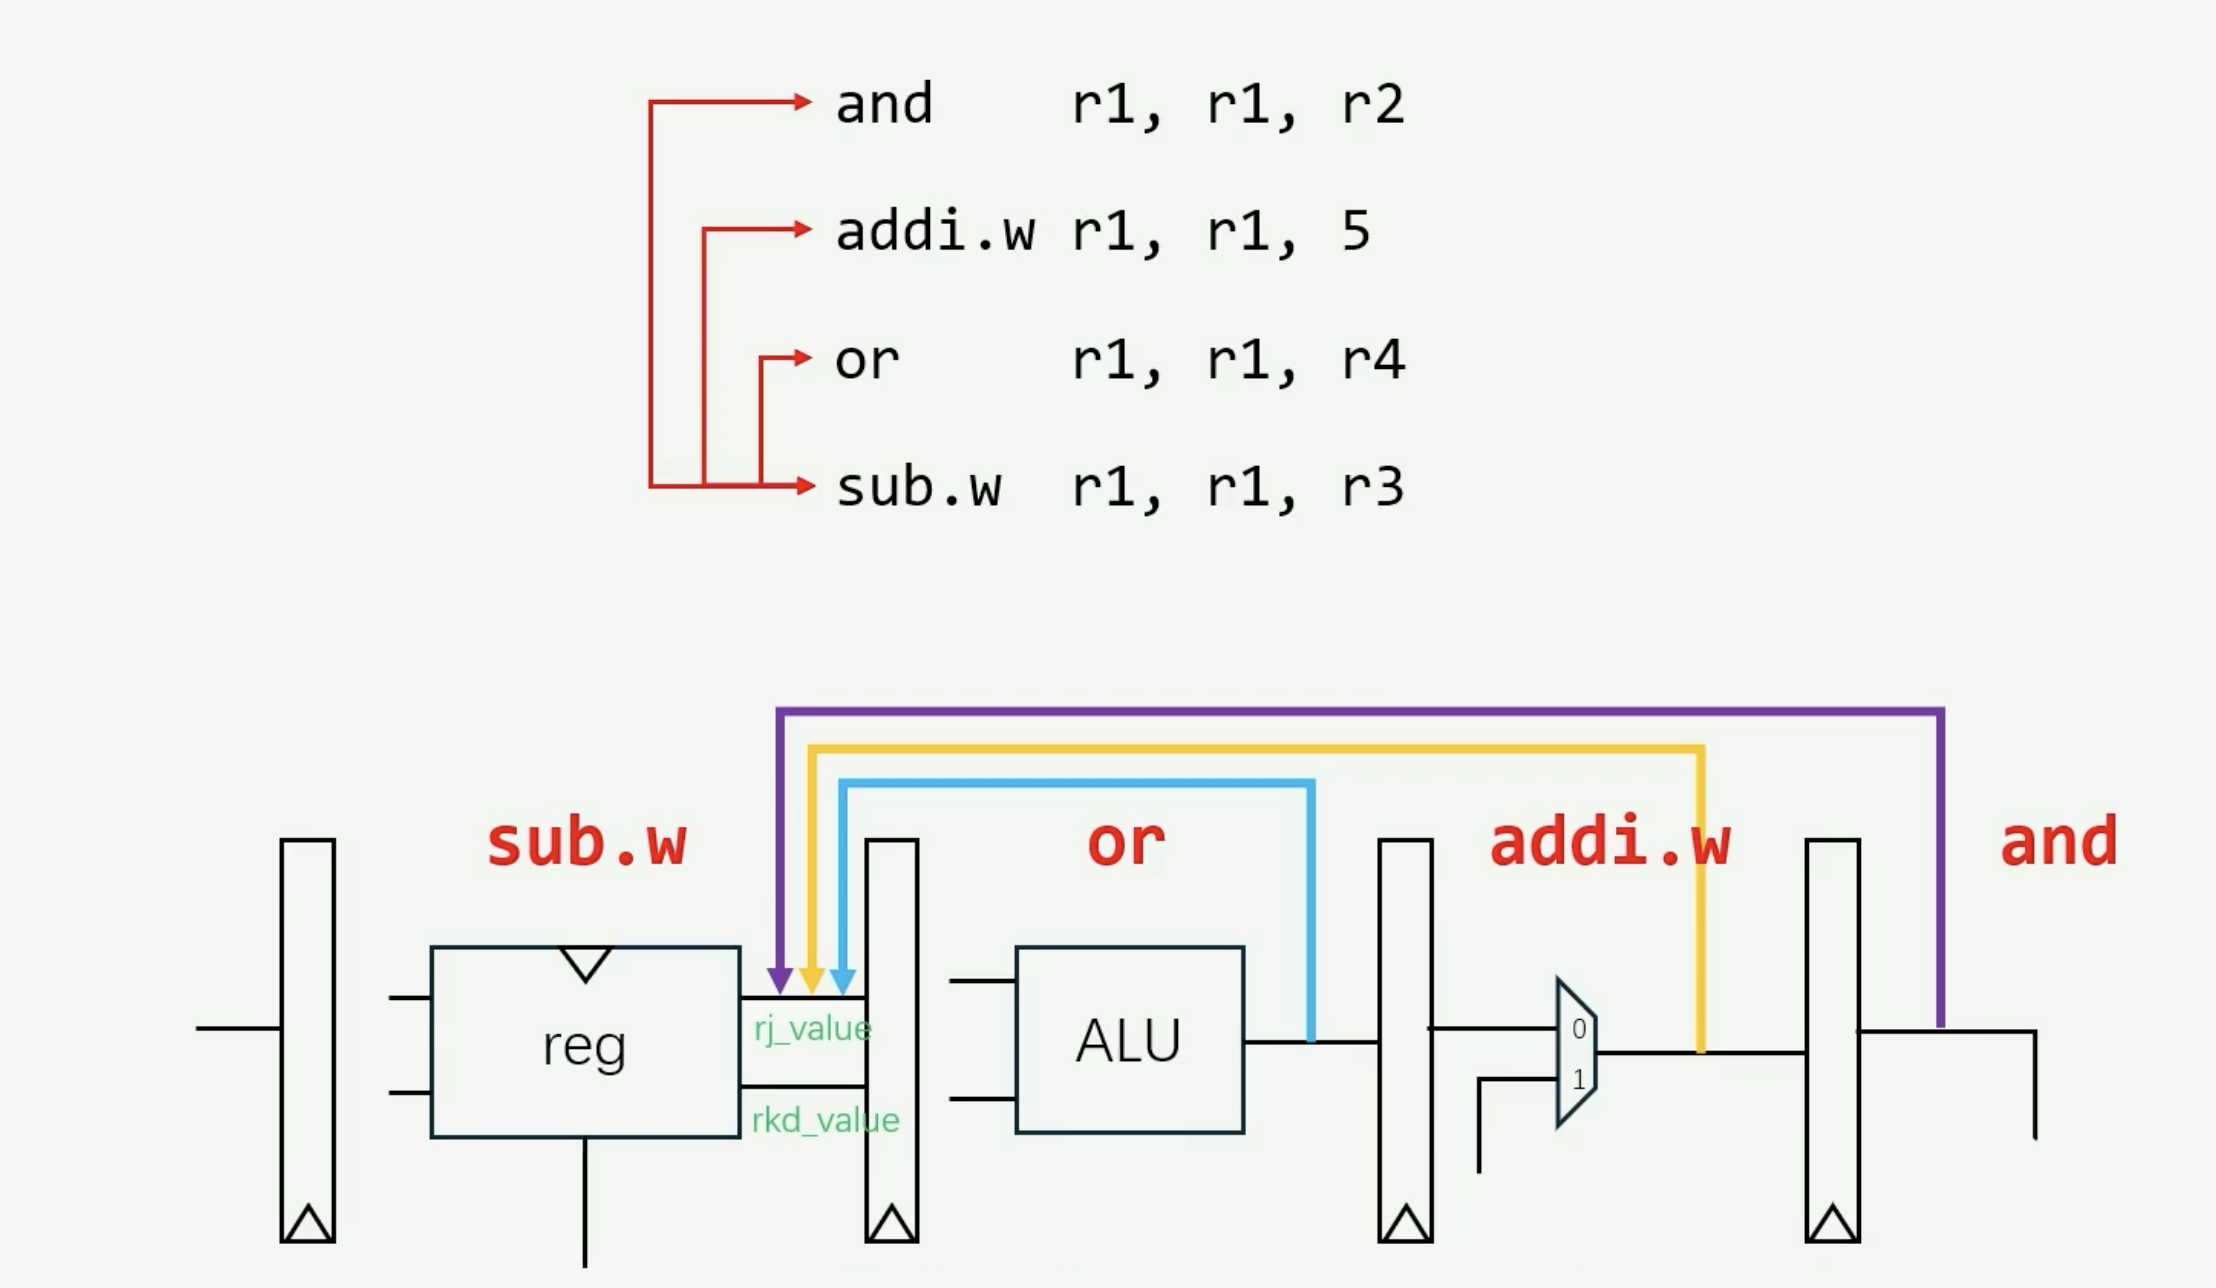
\includegraphics[width=0.8\linewidth]{img/顺序图片/顺序1.png}
    \caption{实现ID阶段的旁路示意图}
\end{figure}

这样就避免了就把所有控制都放在了ID阶段,简化了逻辑。同时我借上图也表达另一个我在实现中个人觉得很需要注意的问题,就是前递有限级别(顺序)。例如EXE和WB阶段都需要前递,\textbf{这时候要优先前递EXE阶段的值,但同时,这也是导致「转移计算未完成」的原因:}


\begin{figure}[H]
    \centering
    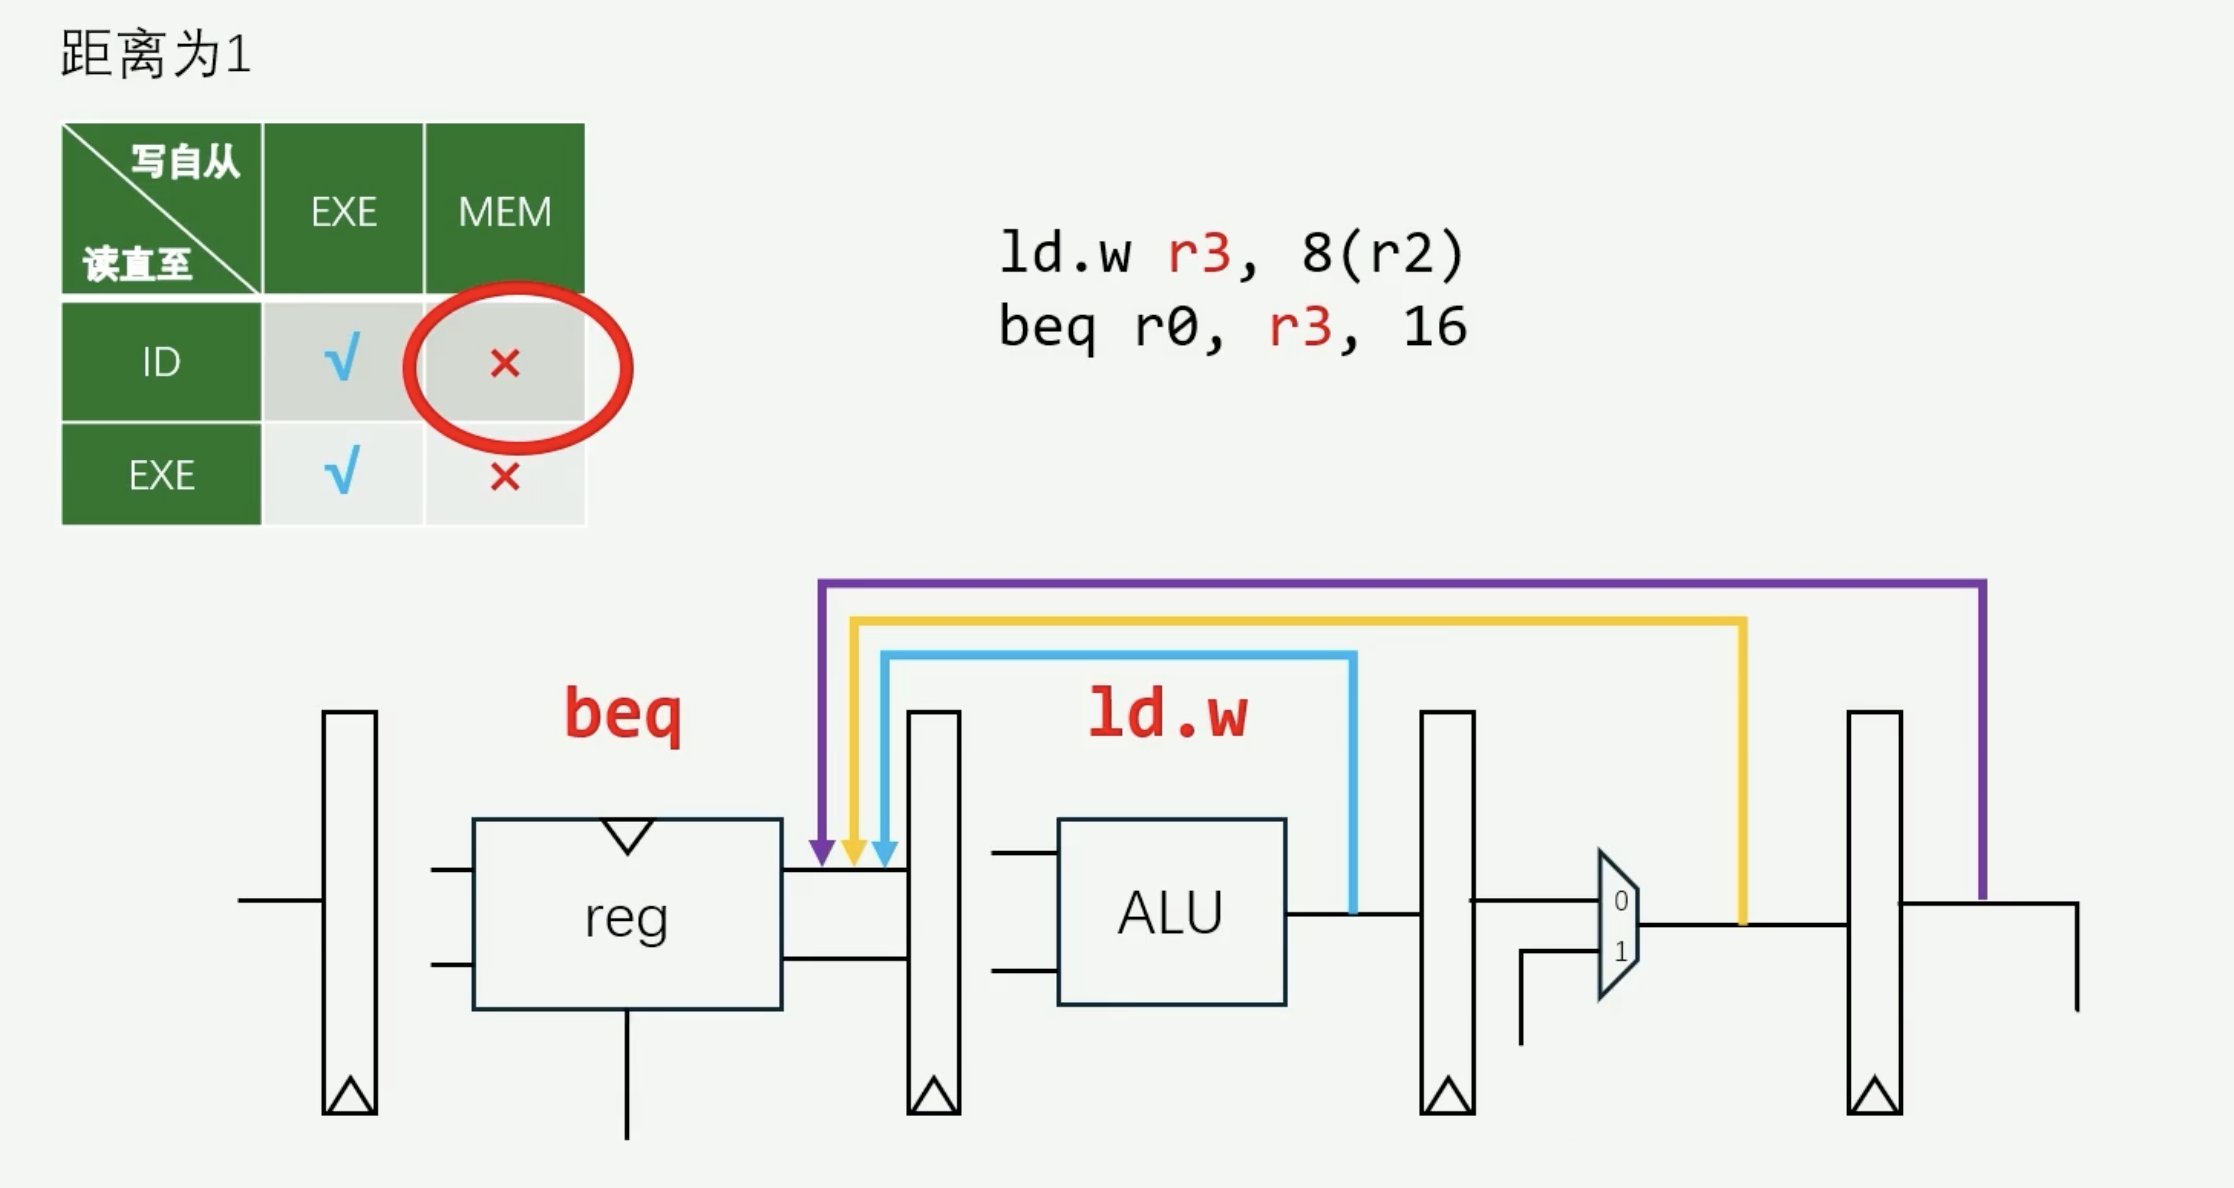
\includegraphics[width=0.8\linewidth]{img/顺序图片/需要阻塞情况1.png}
    \caption{load-branch类型的出错}
\end{figure}

看该图片,正因采用了每次优先前递EXE阶段的值,才导致了load-branch类型的出错。

\begin{figure}[H]
    \centering
    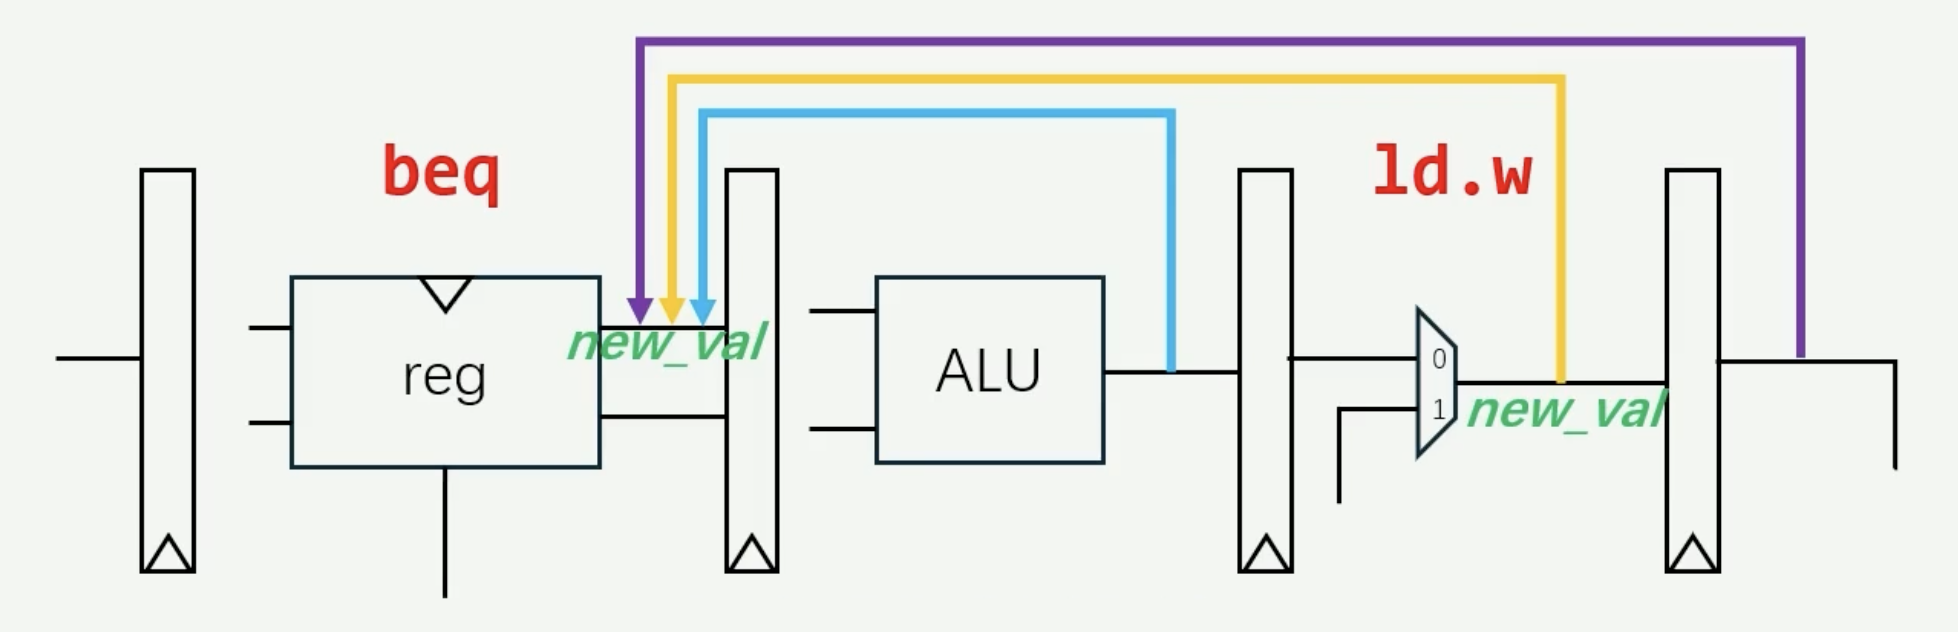
\includegraphics[width=0.8\linewidth]{img/顺序图片/需要阻塞情况2.png}
    \caption{正确实现}
\end{figure}

因此,正确实现应该是发出一个stall信号,使得ld指令执行到MEM阶段,这样就可以解除错误。

\subsubsection{具体判断逻辑}


\begin{lstlisting}[language=Verilog,caption={是否出现相关性}]
    // RS寄存器旁路检测
    wire exe_bypass_rs = EXE_valid & (rs != 5'd0) & (rs == EXE_wdest);
    wire mem_bypass_rs = MEM_valid & (rs != 5'd0) & (rs == MEM_wdest) & ~exe_bypass_rs;
    wire wb_bypass_rs  = WB_valid & (rs != 5'd0) & (rs == WB_wdest) & ~exe_bypass_rs & ~mem_bypass_rs;
    // 同理于rt寄存器
\end{lstlisting}

如果后面的阶段有效,且不是0寄存器,且写回地址与rs/rt相同,则认为出现相关性。

\begin{lstlisting}[language=Verilog,caption={旁路源编码(优先级检测)}]
output [1:0] rs_bypass_source,     // rs旁路源 (00:无, 01:EXE, 10:MEM, 11:WB)
output [1:0] rt_bypass_source      // rt旁路源 (00:无, 01:EXE, 10:MEM, 11:WB)

// 旁路源编码
assign rs_bypass_source = exe_bypass_rs ? 2'b01 :
                         mem_bypass_rs ? 2'b10 :
                         wb_bypass_rs  ? 2'b11 : 2'b00;
// 同理与rt
\end{lstlisting}

由于上文提及了,如果EXE与后面的阶段同时有相关性,则优先级:EXE > MEM > WB > 寄存器堆。具体设计为了00为无相关,01:EXE, 10:MEM, 11:WB。用于控制我在图2.1中画出的两个MUX。

\newpage

\subsection{实现代码}


\subsubsection{旁路单元详细实现}

\begin{lstlisting}[language=Verilog,caption={模块}]
    module bypass_unit(
        // 当前指令信息
        input [4:0] rs,                    // 源寄存器1地址
        input [4:0] rt,                    // 源寄存器2地址
        input [31:0] rs_value,             // 源寄存器1原始值
        input [31:0] rt_value,             // 源寄存器2原始值
        
        // 后续流水级信息
        input EXE_valid,                   // EXE级有效
        input MEM_valid,                   // MEM级有效
        input WB_valid,                    // WB级有效
        input [4:0] EXE_wdest,             // EXE级写回目标寄存器
        input [4:0] MEM_wdest,             // MEM级写回目标寄存器
        input [4:0] WB_wdest,              // WB级写回目标寄存器
        input [31:0] EXE_result,           // EXE级结果
        input [31:0] MEM_result,           // MEM级结果
        input [31:0] WB_result,            // WB级结果
        
        // 指令类型信息(用于特殊处理)
        input inst_load,                   // 当前指令Load指令
        input inst_mult,                   // 当前指令乘法指令
        input inst_mfhi,                   // 当前指令MFHI指令
        input inst_mflo,                   // 当前指令MFLO指令
        input inst_mfc0,                   // 当前指令MFC0指令
        
        // EXE级指令类型信息(用于Load-Use相关检测)
        input EXE_inst_load,               // EXE级Load指令
        input EXE_inst_mult,               // EXE级乘法指令
        
        // 旁路结果输出
        output [31:0] bypassed_rs_value,   // 旁路后的rs值
        output [31:0] bypassed_rt_value,   // 旁路后的rt值
        
        // 控制信号输出
        output stall_required,             // 需要阻塞信号
        output rs_bypass_valid,            // rs旁路有效
        output rt_bypass_valid,            // rt旁路有效
        output [1:0] rs_bypass_source,     // rs旁路源 (00:无, 01:EXE, 10:MEM, 11:WB)
        output [1:0] rt_bypass_source      // rt旁路源 (00:无, 01:EXE, 10:MEM, 11:WB)
    );    
\end{lstlisting}

虽然这个比较占地方,但是由于本次实验主要就是这个代码,因此依然还是把声明(所有接口)原封不动给出了。主要的特殊信息就是load和乘法累指令,还有协处理器指令:inst\_mfc0。 


\begin{lstlisting}[language=Verilog,caption={阻塞控制信号-产生}]
// 需要阻塞的情况
assign stall_required = load_use_hazard_rs | load_use_hazard_rt | 
                       mult_use_hazard_rs | mult_use_hazard_rt;
\end{lstlisting}

需要阻塞的情况就是乘法和load,协处理器情况不需要阻塞,因为都会cancel掉,所有valid值应该都在cancel信号的控制下。


\begin{lstlisting}[language=Verilog,caption={阻塞控制信号-细节}]
// Load-Use相关:EXE级Load指令的结果需要2个周期才能获得
wire load_use_hazard_rs = exe_bypass_rs & EXE_inst_load;
wire load_use_hazard_rt = exe_bypass_rt & EXE_inst_load;
// 多周期操作相关:EXE级乘法指令需要多周期完成
wire mult_use_hazard_rs = exe_bypass_rs & EXE_inst_mult;
wire mult_use_hazard_rt = exe_bypass_rt & EXE_inst_mult;
\end{lstlisting}

因此,具体实现的两个信号是这样的,主要有相关性,且EXE阶段(注意不是本阶段)的指令运行的事乘法或者load,都需要stall。

\begin{lstlisting}[language=Verilog,caption={阻塞控制信号-效果}]
    // assign rs_wait = ~inst_no_rs & (rs!=5'd0) & ( (rs==EXE_wdest) | (rs==MEM_wdest) | (rs==WB_wdest) );
    // assign rt_wait = ~inst_no_rt & (rt!=5'd0)  & ( (rt==EXE_wdest) | (rt==MEM_wdest) | (rt==WB_wdest) );
    assign ID_over = ID_valid & (~inst_jbr | IF_over) & ~stall_required;
\end{lstlisting}

删除掉原先的rs/rt\_wait信号,而是用我新定义的stall来控制ID是否over(ready\_go) 。如果ID没有ready\_go,那么由于:
\begin{lstlisting}[language=Verilog,caption={级联控制}]
    assign IF_allow_in  = (IF_over & ID_allow_in) | cancel;
    assign ID_allow_in  = ~ID_valid  | (ID_over  & EXE_allow_in);
\end{lstlisting}

所以ID阶段被阻塞,IF阶段无法进入;这样就成功解决了错误情况(完成阻塞)。


\subsubsection{总线传递与模块接口变化}

最开始我的实现修改了总线信号,后来思考为了简便与清晰性,可以考虑单独抽出一些信号:
\begin{lstlisting}[language=Verilog,caption={decoder新添加的信号}]
// 旁路数据输入
input      [ 31:0] EXE_result,  // EXE级结果
input      [ 31:0] MEM_result,  // MEM级结果
input      [ 31:0] WB_result,   // WB级结果
// EXE级指令类型信息(用于Load-Use相关检测)
input              EXE_inst_load,  // EXE级Load指令
input              EXE_inst_mult,  // EXE级乘法指令
\end{lstlisting}

由于旁路模块是在decoder中实例化的,因此其他所有模块都应给Decoder传入相关的信号(如有效值与具体值)。这个具体值需要找到最最后面的,具有决定性的值,以WB阶段举例:

\begin{lstlisting}[language=Verilog,caption={WB阶段向前传递的result}]
    assign rf_wen   = wen & WB_over;
    assign rf_wdest = wdest;
    assign rf_wdata = mfhi ? hi : mflo ? lo : mfc0 ? cp0r_rdata : mem_result;
    assign WB_result = rf_wdata;  // ! 旁路输出
\end{lstlisting}

除此之外,每个模块的输出也需要增加,以EXE为例:

\begin{lstlisting}[language=Verilog,caption={EXE模块新添加的信号}]
    // 新增旁路数据输出
    output     [ 31:0] EXE_result,   // EXE级结果,用于旁路
    
    // EXE级指令类型信息输出
    output             EXE_inst_load,  // EXE级Load指令
    output             EXE_inst_mult,  // EXE级乘法指令
\end{lstlisting}

最后可以举例说明值是如何被选择的,以ALU为例子:


\begin{figure}[H]
    \centering
    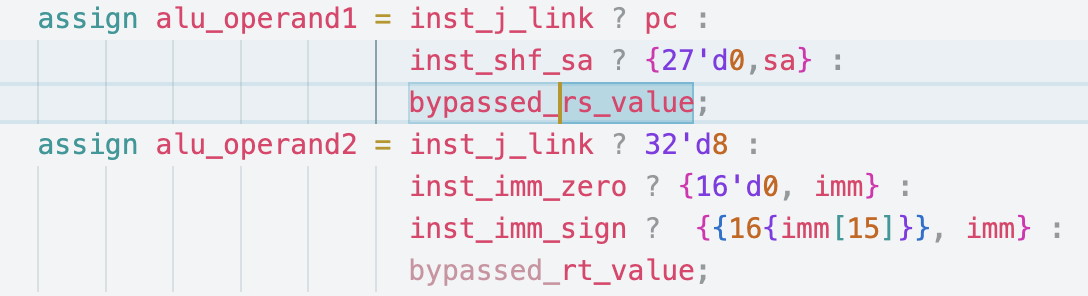
\includegraphics[width=0.8\linewidth]{img/旁路修改图片/alu用旁路的值.png}
    \caption{alu采用旁路值}
\end{figure}

\newpage

\subsection{仿真实验}

\subsubsection{周期变短验证}

下面进行仿真实验,首先整体上可以看到周期变短了,且更加整齐,先前由于级联控制,不同的指令经常因为种种情况导致延迟,现在可以看到只有Beq指令可能遇到延迟(44H-48H):
\begin{figure}[H]
    \centering
    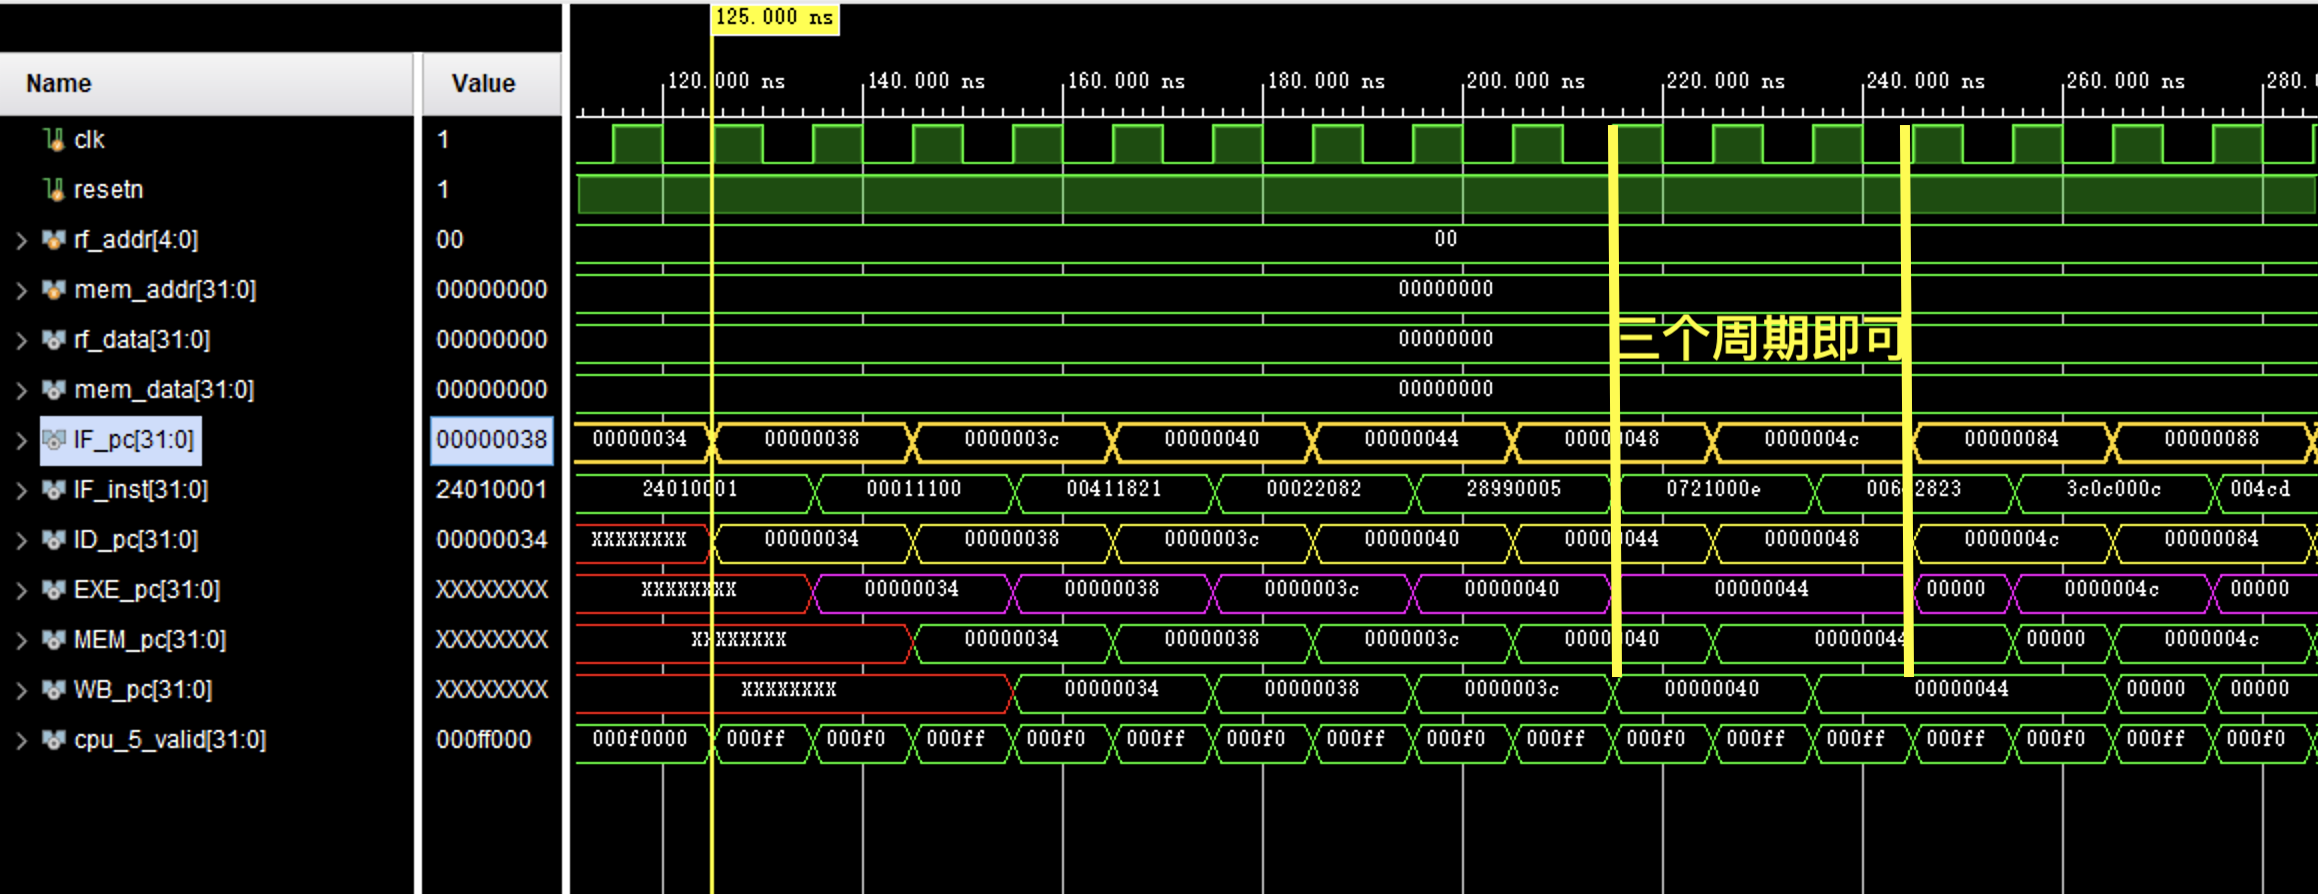
\includegraphics[width=0.9\linewidth]{img/旁路修改图片/明显看到周期变短.png}
    \caption{明显看到周期变短}
\end{figure}

对比之前的,可以看到先前的44占据了4个周期,现在占据三个周期。且其余指令也都有长进(具体见本章最后的举例部分)。

\begin{figure}[H]
    \centering
    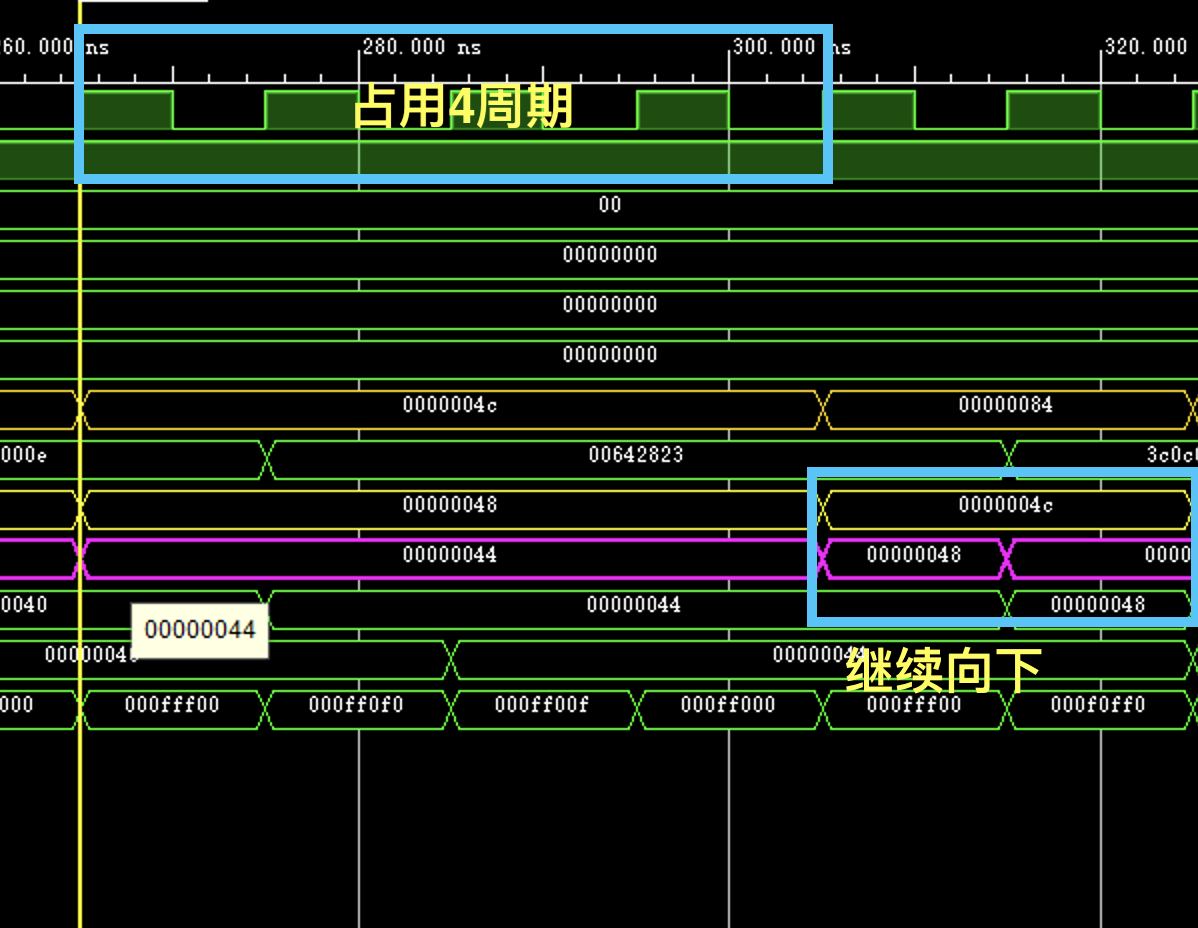
\includegraphics[width=0.9\linewidth]{img/顺序图片/跳转1周期分析.png}
    \caption{先前的跳转1周期分析}
\end{figure}


\subsubsection{延迟情况验证}

延迟情况的话,就是beq指令部分和乘法部分:

\begin{figure}[H]
    \centering
    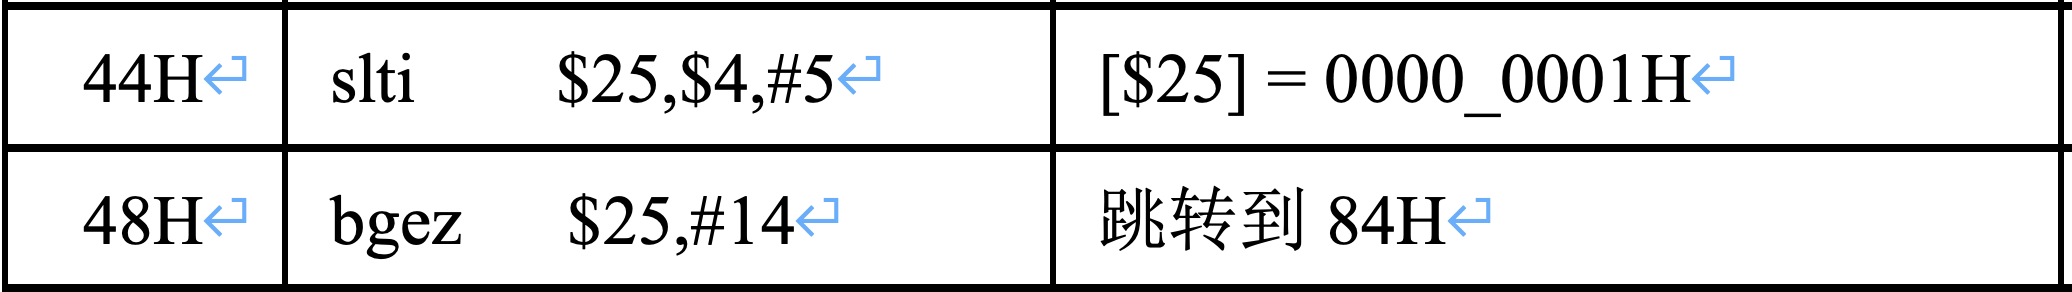
\includegraphics[width=\linewidth]{img/旁路修改图片/beq指令.png}
    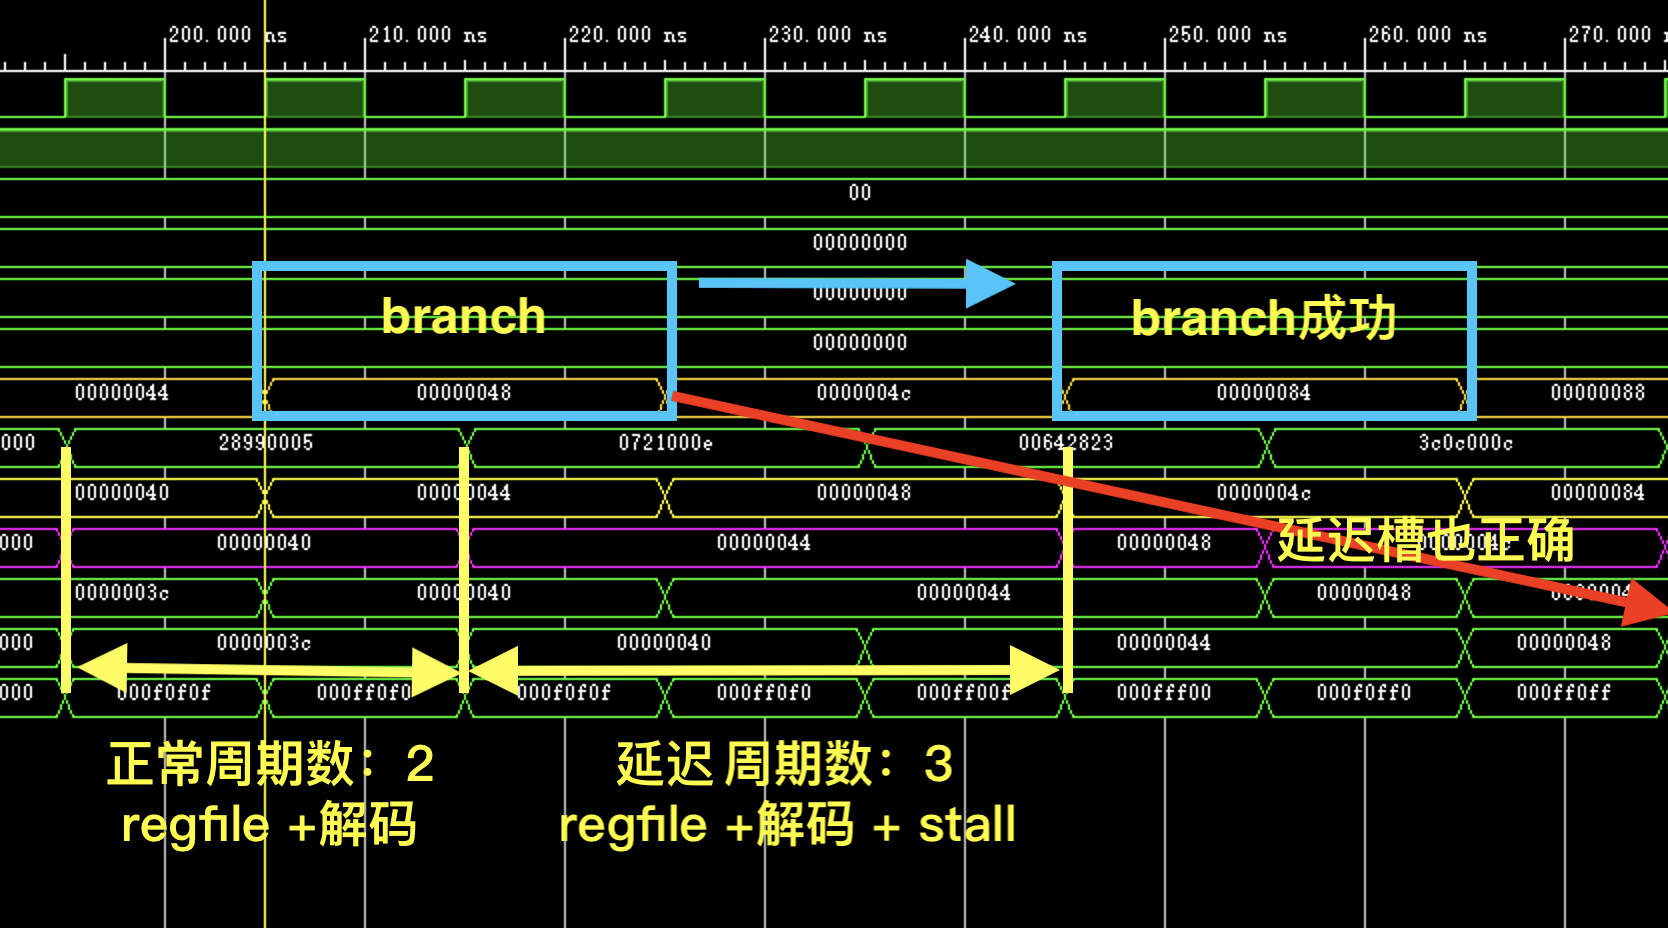
\includegraphics[width=\linewidth]{img/旁路修改图片/beq的时候多延迟一个周期.png}
    \caption{beq的时候多延迟一个周期}
\end{figure}

48H是beq指令,可以看到在他前面的具有相关性的指令多停留了一些,这符合我说的对beq指令的时候单独检测stall的逻辑。

可以对比一下最早我实现的EXE阶段前递版本:

\begin{figure}[H]
    \centering
    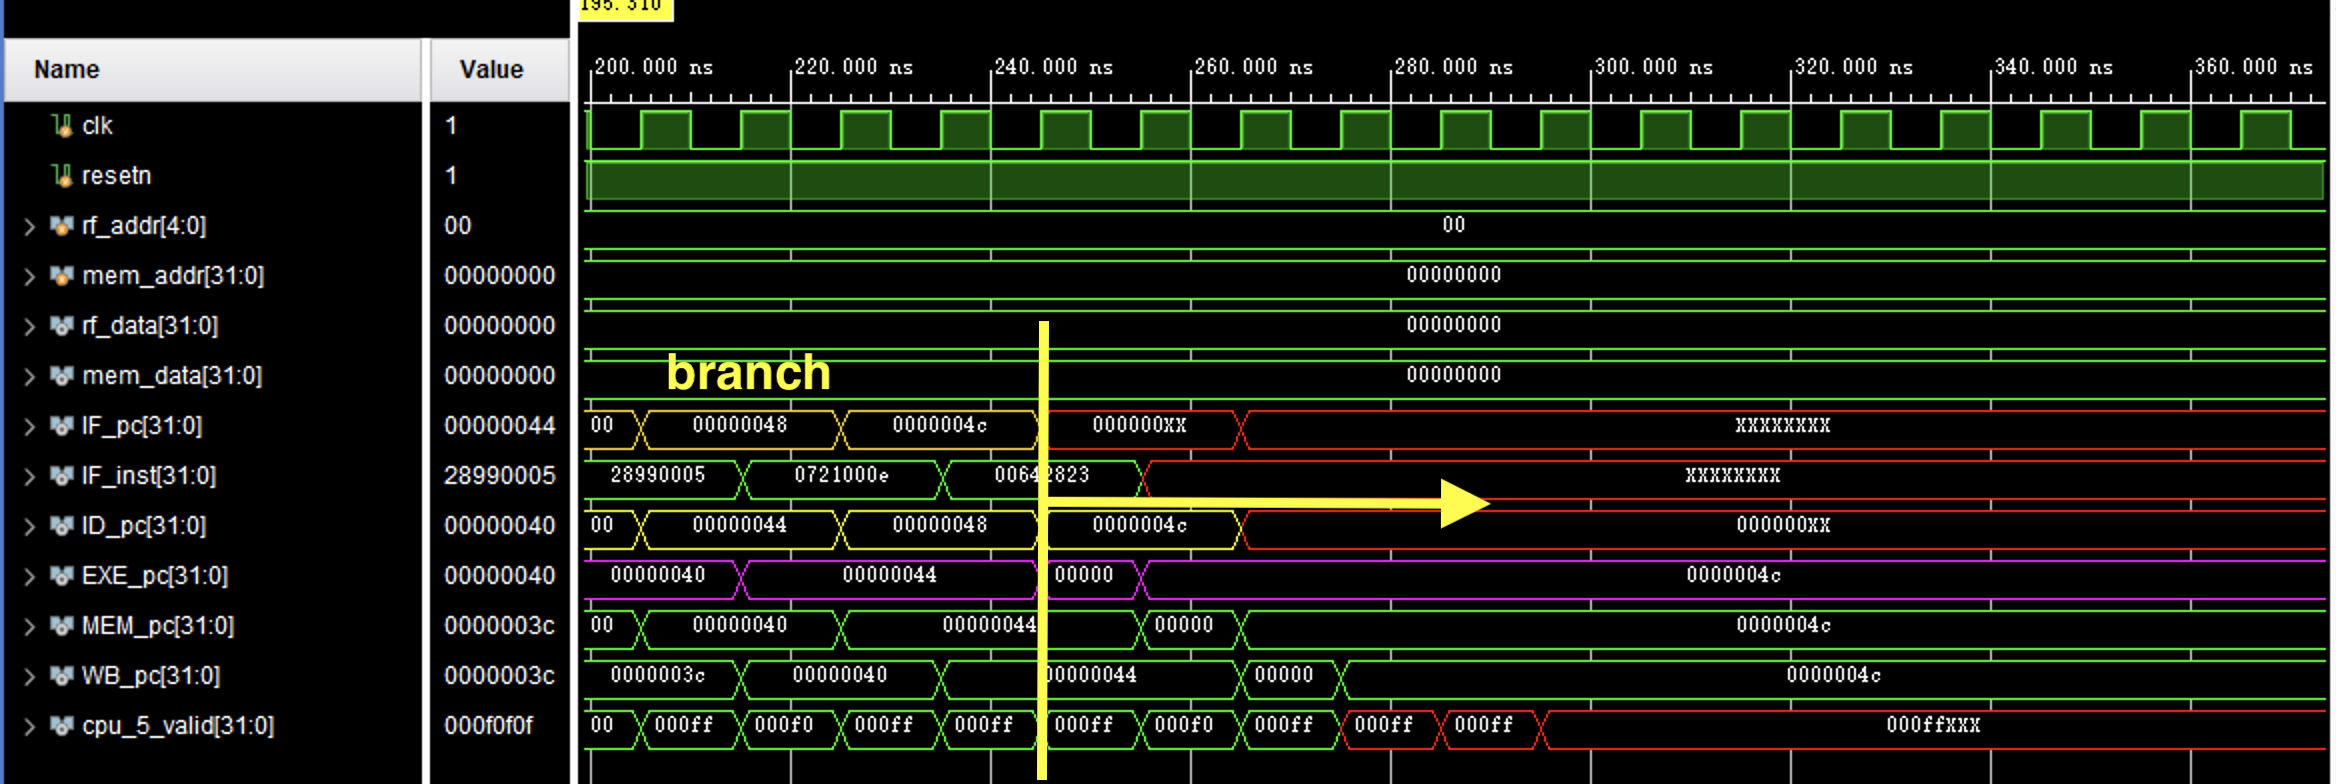
\includegraphics[width=\linewidth]{img/先前错误/增加完EXE阶段旁路2.png}
    \caption{EXE阶段前递版本(最开始的错误实现)}
\end{figure}

这里branch后,虽然前面正常执行,但是branch读到的数值没有定义(一个是有效的值已经随流水走了,另一个是没有处理,即使读到了也是错误的)。



\begin{figure}[H]
    \centering
    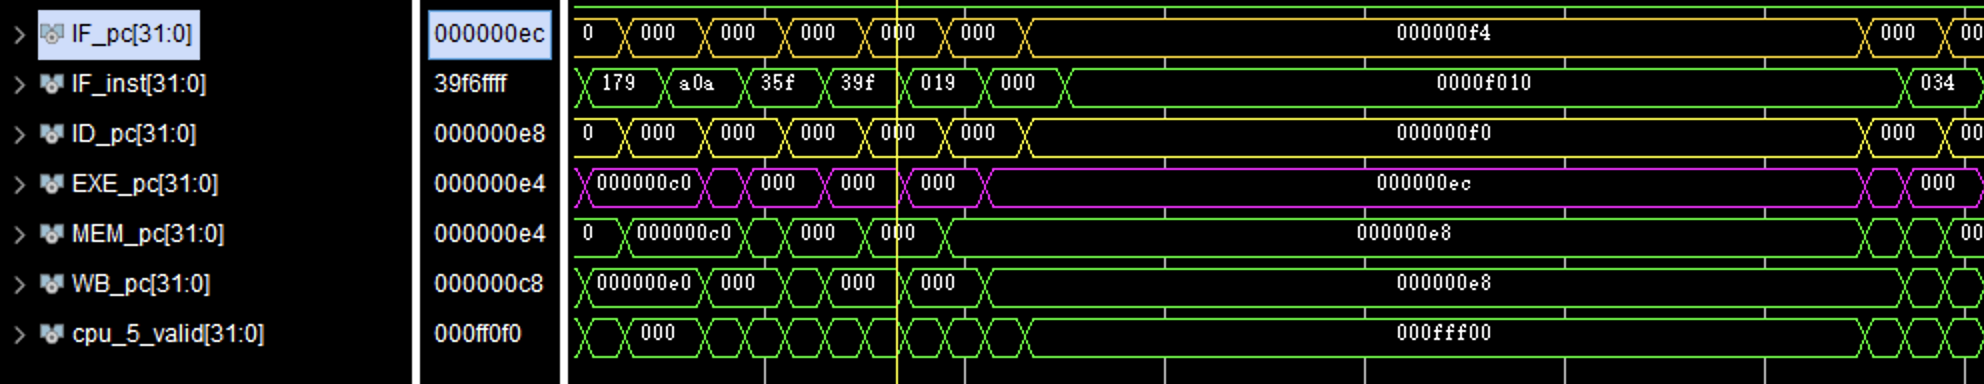
\includegraphics[width=\linewidth]{img/旁路修改图片/乘法情况ech也正常工作.png}
    \caption{乘法也可以正常工作}
\end{figure}
乘法情况,也可以正确控制,如上图,不再赘述。

\subsubsection{最后举例}

最后再举例一个确实减少周期的例子:

54、58H这两个指令,在之前绝对是需要stall的,现在每个都只需要两个周期(regfile+decode,因为这个代码吧regfile单独给了一个周期,我感觉其实没必要,但是表示尊重就没改):


\begin{figure}[H]
    \centering
    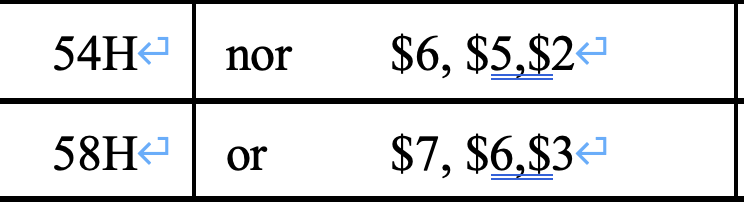
\includegraphics[width=0.5\linewidth]{img/顺序图片/5458H.png}
\end{figure}

\begin{lstlisting}[language=Verilog]
    54H nor $6, $5,$2 
    58H ori $7, $6,$3 // 6具有相关性
\end{lstlisting}


\begin{figure}[H]
    \centering
    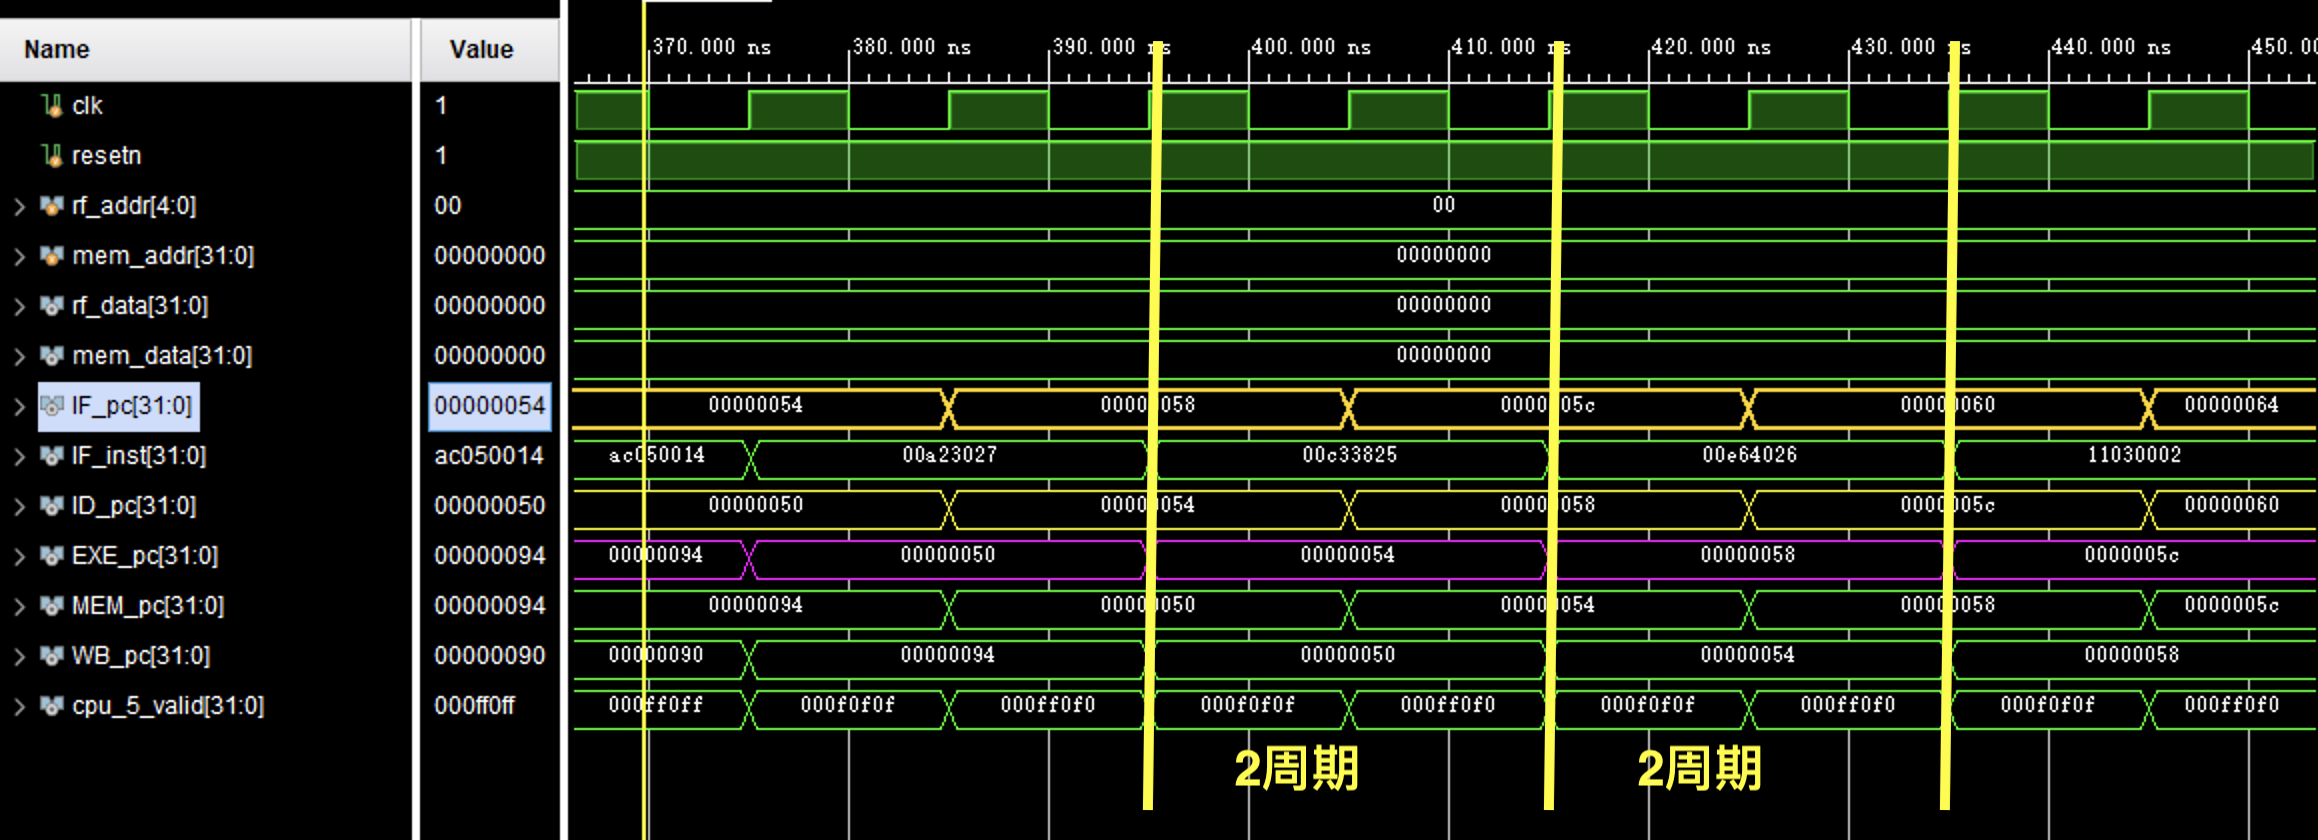
\includegraphics[width=\linewidth]{img/顺序图片/5458.png}
    \caption{54、58H仿真}
\end{figure}

可以看到58H的执行周期完全不受影响,说明旁路在一般情况下确实正确。

\newpage
\section{实验总结与心得体会}

\begin{enumerate}
    \item 最开始实现了不完全正确的旁路(EXE阶段),主要是因为在国庆前,我没有想到ID阶段的branch(课上的版本branch是在EXE阶段),但是后退版本,实现了全部前递到ID阶段的旁路,简化了逻辑。最终正确实现了。
    \item CPU设计那个书也给了我一些灵感,主要是load-branch的处理,但是我并没有采用CPU设计书中的去更改ready\_go(代码中叫做over)信号。而是采用了一个新的stall信号,我认为这样更加清晰和简单,主要还是这样能够实现的情况下,冒险去改级联控制的ready\_go信号,很容易出错。而且很明显可以观察到之前代码中stall产生信号和CPU设计实战那本书中建议的修改方法是冲突的,只能留一个,因此我还是选择留stall信号,维护也方便。
    \item 实现代码中,我认为比较需要注意的点就是前递有限级别(顺序),和stall信号的产生。前者既保证了旁路的正确,但同时也产生了load-branch类型的错误,我认为我报告的一个优点也在于解释了转移计算未完成的原因(CPU设计实战那本书中没有提到)。
    \item 感觉有点难度。
\end{enumerate}
    

\label{LastPage}

\end{document}
